\section{Introduction}
RDF identifies resources using IRIs and represents their relations as triples~\cite{rdf11}. SPARQL provides expressive graph access~\cite{sparql11}, but users often begin with a name rather than an identifier or knowledge of the vocabulary. They need to find the corresponding resource before inspecting its graph context and the information available from other endpoints.

\tp{} connects discovery and exploration through a shared IRI. Maintainers select searchable metadata for a local catalog and provide reusable SPARQL queries; users find an entity and open its actions without writing SPARQL. Discovery terminology can be curated independently of graph literals, while query actions remain under the interface maintainer's control.

The system integrates (i) a catalog-to-IRI-to-query workflow, (ii) catalog generation and transactional import, and (iii) file-based query actions with RDF, media, and location views. This is an interface contribution, not a new indexing or federation algorithm. Source and documentation are available online.\footnote{\url{https://github.com/dice-group/triple-peek}; documentation: \url{https://dice-group.github.io/triple-peek/}.}

\paragraph{Related work.}
YASGUI supports SPARQL editing and result visualization~\cite{yasgui2017}, whereas \tp{} starts from catalog search and exposes operator-defined actions. LodView renders navigable HTML views of RDF resources~\cite{lodview}; \tp{} adds a separately maintained discovery catalog. SemFacet supports semantic faceted search and interactive query refinement~\cite{semfacet2014}, while \tp{} exposes fixed entity-anchored templates. These are differences in interaction models, not evidence of comparative effectiveness.

\section{Architecture and Data Flow}
Figure~\ref{fig:workflow} shows the architecture. The \emph{search layer} maps text to records; the \emph{application} displays candidates and instantiates actions; the \emph{endpoint} executes queries and any configured federation. The implementation uses TypeScript, Next.js, React, PostgreSQL, N3.js, and MapLibre GL. Docker Compose separates the database, application, catalog generator, and importer.

\begin{figure*}[t]
  \centering
  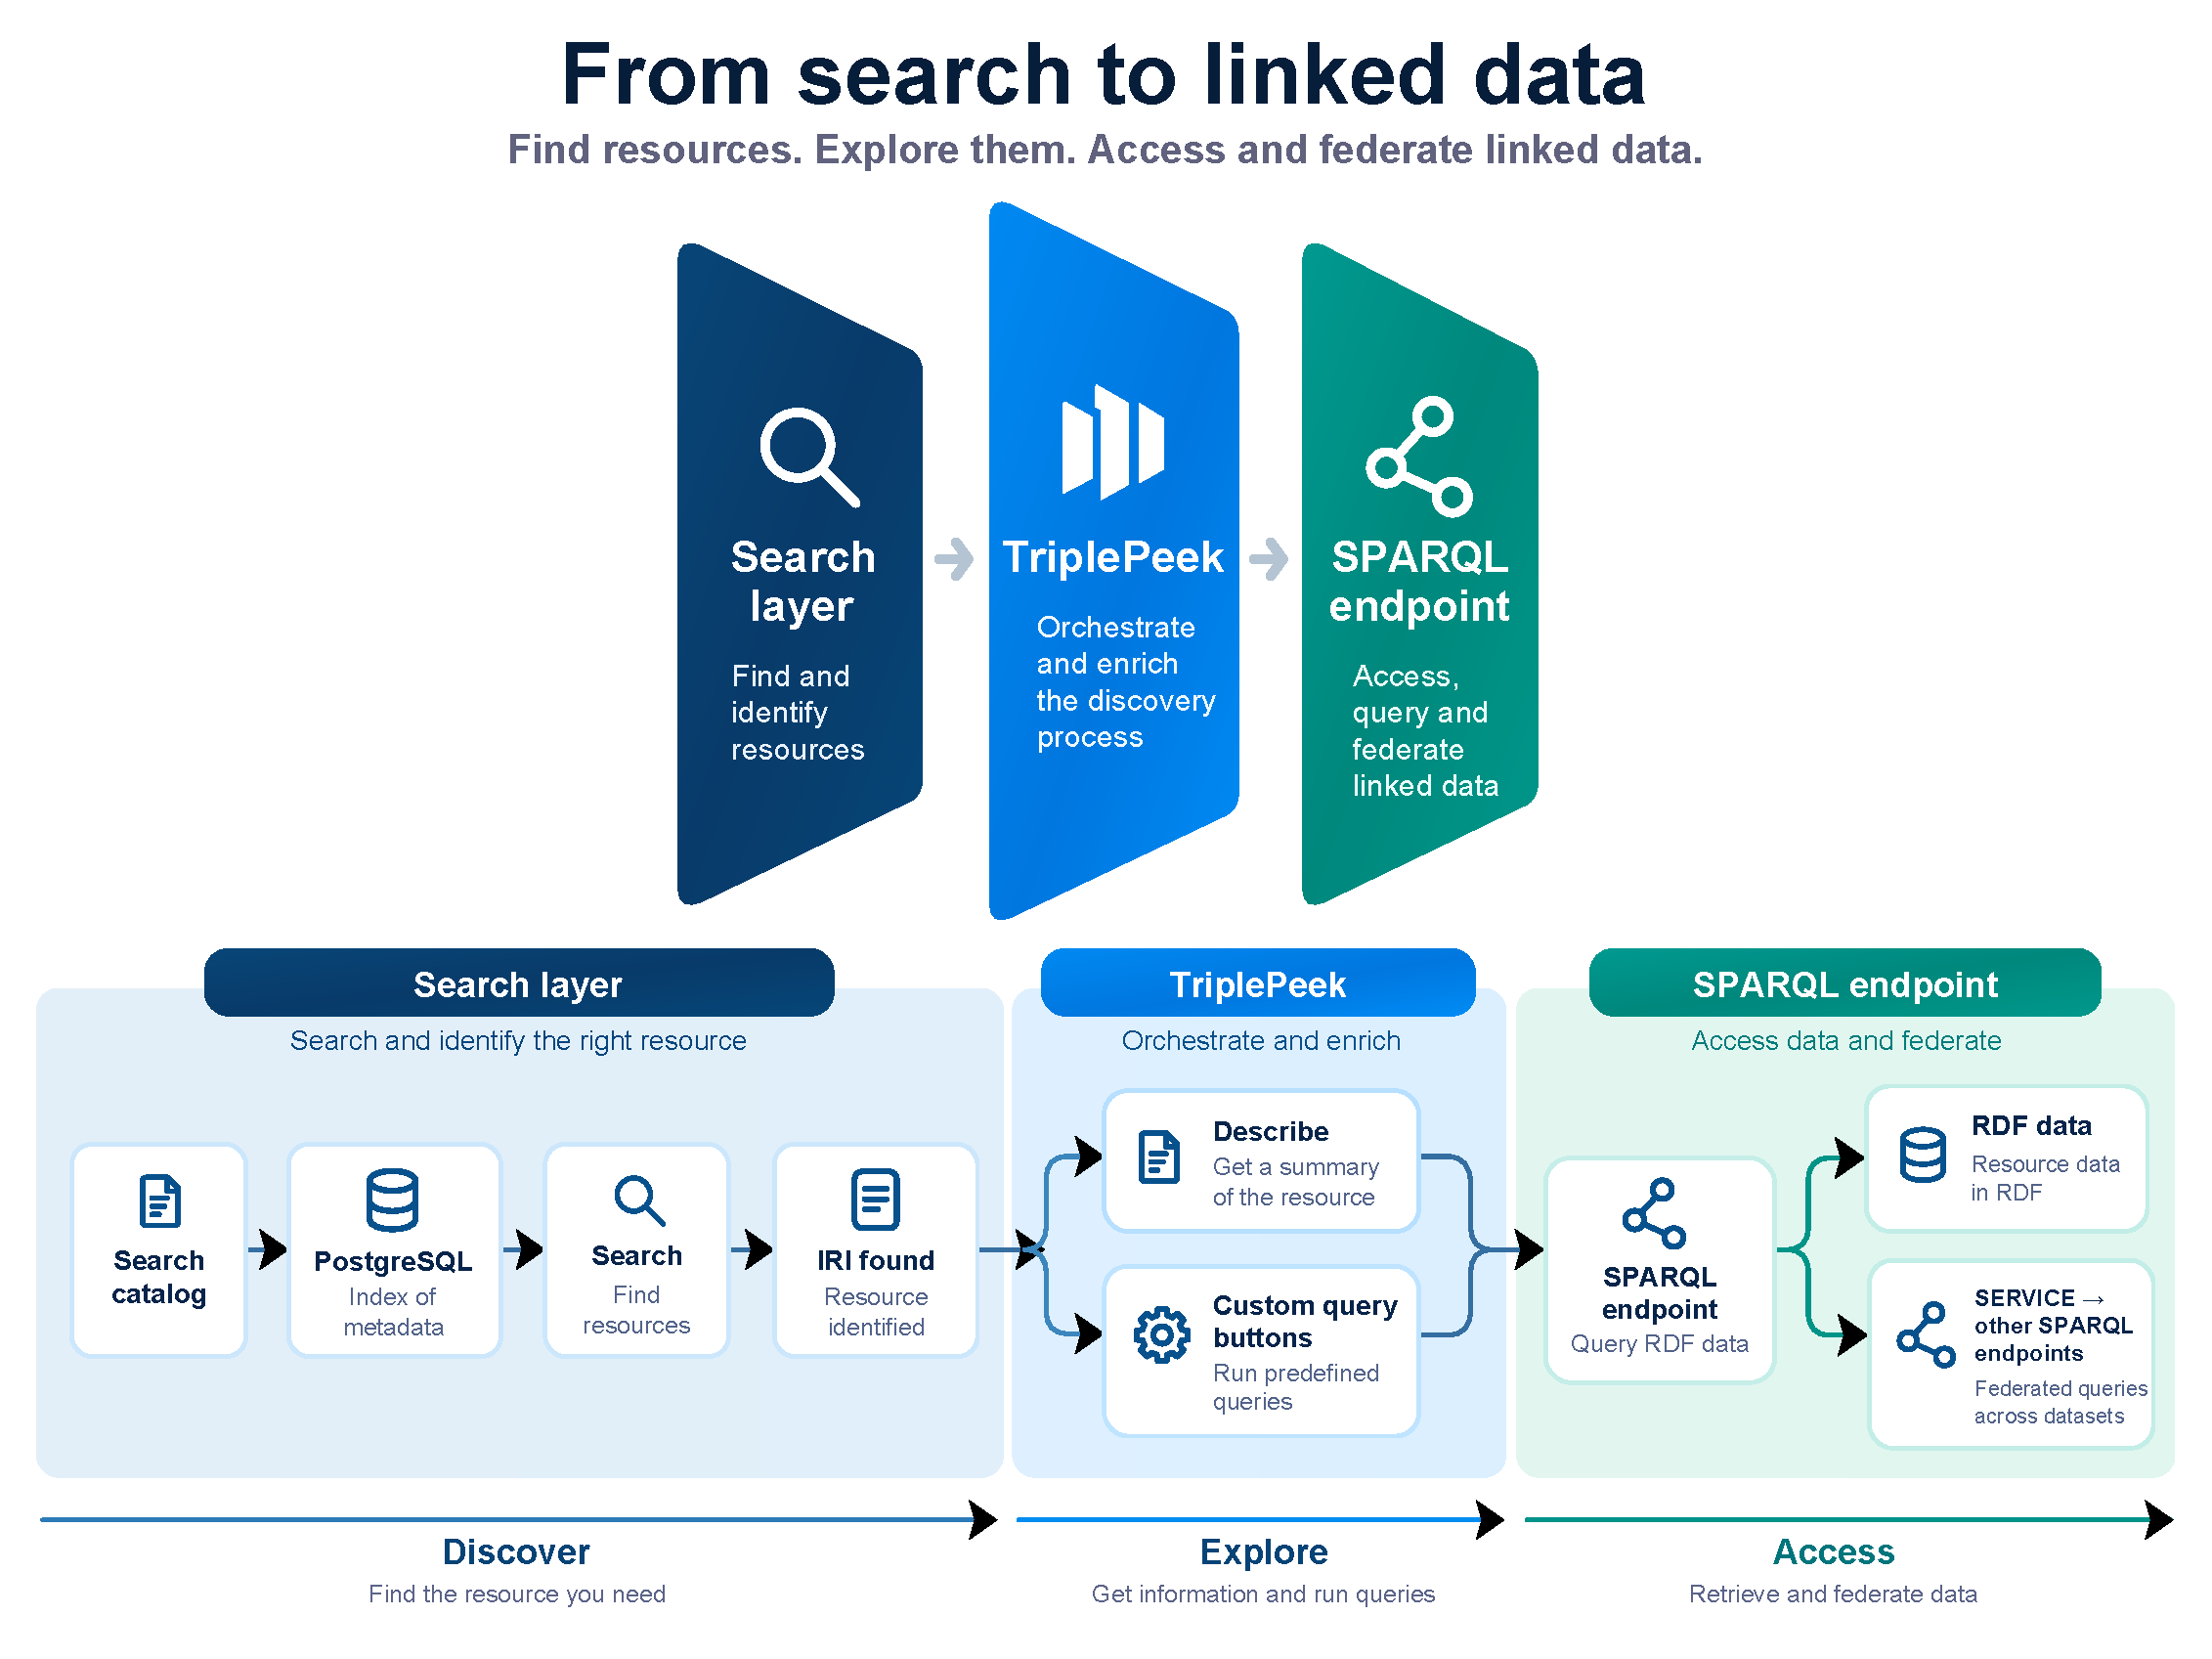
\includegraphics[width=0.91\textwidth]{figures/how-it-works.pdf}
  \caption{\tp{} workflow. Catalog search identifies an IRI; the application then requests a description or instantiates a query template. SERVICE clauses are executed by the configured endpoint. Responses may be RDF graphs, SELECT bindings, or ASK booleans. ``Summary'' denotes an endpoint-defined DESCRIBE result.}
  \Description{The search catalog is imported into PostgreSQL. Search returns a resource IRI, which flows to either Describe or a custom query button. Both actions contact the primary SPARQL endpoint. That endpoint returns data or invokes other endpoints through SERVICE.}
  \label{fig:workflow}
\end{figure*}

Let $E$ be the configured endpoint and $C$ a finite catalog:
\begin{equation}
 C = \{(u,\ell,\mathbf{m})\}, \qquad
 q \longmapsto C_q \longmapsto u \longmapsto
 \operatorname{eval}_{E}(T[u]).
\end{equation}
Here $u$ is a resource IRI, $\ell$ its display label, $\mathbf{m}$ selected textual metadata, $q$ a search string, and $C_q$ the ranked candidates. A selected template $T$ is instantiated with $u$. The built-in action uses \texttt{DESCRIBE <}$u$\texttt{>}. Its returned graph is determined by the endpoint; it is not guaranteed to contain every incident triple.

The catalog is a discovery projection, not an RDF replica. Metadata may combine graph values, alternative terminology, and curated descriptions; its coverage bounds text-search recall. Search requests access PostgreSQL only. Opening an action triggers SPARQL retrieval, so search input changes do not contact the endpoint. This separates workloads without establishing a latency improvement.

\subsection{Catalog Preparation and Import}
A CSV catalog contains at least \texttt{iri} and \texttt{label}; further columns become searchable metadata. Alternatively, the generator executes an operator-provided SELECT query against $E$ and exports bindings using LIMIT/OFFSET pagination. Operators can bound the number of exported rows or the UTF-8 file size. The generator writes complete CSV rows into a temporary file and replaces the destination only after successful export. Stable pagination requires a suitably ordered query and a sufficiently stable endpoint dataset; the bundled query does not enforce either condition.

Before importing, the pipeline normalizes the second column to \texttt{label} and validates headers, CSV structure, and IRIs. When the same IRI occurs in several rows, validation automatically groups the distinct, nonempty values in each field and retries validation. Thus, multiple type labels can be aggregated into one field alongside the resource label in a single catalog row per IRI. A PostgreSQL staging table holds validated rows. Schema changes, index creation, and insertion occur within one transaction, so an import failure leaves the search table unchanged. File normalization occurs separately and can modify the CSV.

By default, an IRI already present in the table causes insertion to fail. With \texttt{--update}, incoming rows replace searchable values for the corresponding IRIs; omitted metadata columns become NULL and absent IRIs remain unchanged. The importer creates a full-text GIN index, a trigram GIN index, and an index on lower-case labels for prefix matching. All imported fields, including the IRI, contribute to the generated search text.

\subsection{Entity Search and Ranking}
Candidate retrieval combines exact labels, label prefixes, full-text matching, and trigram word similarity. Let $x_c$ be the concatenated fields of a record $c$ and $v_c$ its PostgreSQL text-search vector. The priority of a matching record is the first satisfied condition:
\begin{equation}
 p(c,q)=\begin{cases}
 1 & \text{case-insensitive exact label},\\
 2 & \text{case-insensitive literal label prefix},\\
 3 & \text{full-text match against }v_c,\\
 4 & \text{trigram word-similarity match against }x_c.
 \end{cases}
\end{equation}
Full-text matching uses \path|plainto_tsquery| with the \texttt{simple} configuration. Within priorities 1--3, the score is \path|ts_rank_cd|; within priority 4, it is \path|word_similarity|~\cite{pgtext,pgtrgm}. Trigram eligibility uses PostgreSQL's configured word-similarity threshold. No learned model or embedding search participates in this ranking.

Results are ordered by ascending priority, descending score, lower-case label, original label, and IRI. A keyset cursor records this ordering tuple and the query string. The API returns at most 20 records per page and deduplicates by IRI before limiting. The interface waits 300\,ms after an input change before requesting a page. Result cards show the label, IRI, and bounded metadata summaries; metadata too long to display can still contribute to search.

\subsection{Query Actions and Presentation}
Each regular \texttt{.sparql} file in the application's buttons directory defines an action. Templates use the literal placeholder \texttt{\$\{iri\}} inside an IRI reference. For example, the following entity-summary action retrieves an image and coordinates:
\begin{lstlisting}
PREFIX wdt: <http://www.wikidata.org/prop/direct/>
SELECT ?image ?coord WHERE {
  OPTIONAL { <${iri}> wdt:P18 ?image }
  OPTIONAL { <${iri}> wdt:P625 ?coord }
}
\end{lstlisting}
The server validates the supplied IRI, substitutes all placeholders, and recognizes SELECT, ASK, CONSTRUCT, or DESCRIBE after prefix/base declarations. Templates are trusted operator configuration; update forms are unsupported. Requests use the configured endpoint and a 15-second timeout. SELECT and ASK request SPARQL JSON results; graph queries prefer Turtle. A template may include SERVICE clauses, whose execution and remote-source access are delegated to the endpoint~\cite{sparql11}.

Parseable RDF graph responses are displayed as subject--predicate--object tables, with a graph column where applicable. Selecting a named RDF term reruns the panel's action for that IRI, and a local history supports backward navigation. SELECT results are grouped into distinct values per projected variable, and ASK results appear as booleans. Grouping suits entity attributes but does not preserve correlations between variables across result rows. Recognized image URLs and point coordinates add media previews and map markers; these views are heuristic interpretations of returned values.

\section{Demonstration and Evidence}
\paragraph{Scenario.}
The bundled Wikidata catalog contains 10,000 rows and 10,000 distinct IRIs with four fields: IRI, label, type label, and country. These counts were obtained directly from the distributed CSV. Its generation query selects castles with English labels, an image, and coordinates, enriching them with type and country labels. A visitor searches for \emph{Neuschwanstein Castle}, identifies the resource, and opens Describe to inspect its graph. The Details action requests an image, coordinates, and an English description. The Embedding action uses SERVICE to retrieve a precomputed Keci embedding from a separate endpoint. It demonstrates cross-source retrieval, not embedding generation or similarity search. Live results depend on the configured services and may differ from catalog metadata.

\paragraph{Endpoint interoperability.}
We successfully tested DESCRIBE against all six endpoints in Table~\ref{tab:endpoints}, covering embeddings, general knowledge, and research software. SemRepo links GitHub repositories to their scholarly context~\cite{semrepo2026}. Selected custom actions described above were also exercised, without asserting every action on every endpoint. Responses appeared immediate during manual use; no endpoint latency measurements are reported. Earlier exploratory use additionally included a DICE university corpus and Fuseki, for which endpoint details remain unspecified.

\begin{table*}[t]
\centering
\caption{Endpoints tested with DESCRIBE. DICE snapshot and Tentris version information was supplied by the authors. Linked service documentation identifies the public-service backends; their tested versions were not supplied.}
\label{tab:endpoints}
\begin{tabular}{@{}p{0.41\textwidth}p{0.35\textwidth}p{0.15\textwidth}@{}}
\toprule
Endpoint & Dataset or snapshot & Backend \\
\midrule
\url{https://sparql.embeddings.cc/sparql} & DBpedia and Wikidata embeddings & Tentris 1.0.0 \\
\url{https://dbpedia.data.dice-research.org/sparql} & \href{https://databus.dbpedia.org/dbpedia/collections/dbpedia-snapshot-2022-12}{DBpedia snapshot 2022-12} & Tentris 1.0.0 \\
\url{https://wikidata.data.dice-research.org/sparql} & \href{https://dumps.wikimedia.org/wikidatawiki/entities/20250122}{Wikidata 2025-01-22 truthy beta} & Tentris 1.0.0 \\
\url{https://query.wikidata.org/sparql} & Official Wikidata Query Service & \href{https://wikitech.wikimedia.org/wiki/Wikidata_query_service/Runbook}{Blazegraph} \\
\url{https://dbpedia.org/sparql} & Official DBpedia public endpoint & \href{https://www.dbpedia.org/resources/sparql/}{Virtuoso} \\
\url{https://semrepo.org/sparql} & GitHub repositories linked to research & \href{https://semrepo.org/sparql}{Virtuoso} \\
\bottomrule
\end{tabular}
\end{table*}

\paragraph{Large-catalog observations.}
TriplePeek and PostgreSQL ran in separate Docker Compose containers on one VM with eight CPU cores and 32\,GB RAM. Its catalog held 20 million entities, one row per entity with labels and aggregated types. While typing \emph{Berlin place}, six browser Network-panel search-request durations were 502, 52, 42, 83, 184, and 124\,ms (range 42--502\,ms; median 103.5\,ms). These HTTP durations include the browser--application exchange, exclude the 300\,ms pre-request debounce, and measure neither SQL alone nor remote SPARQL execution. They sample one typing session, not repeated identical queries. Exact prefixes, cache state, storage, and concurrency were not supplied; representative latency and throughput require a controlled workload.

\paragraph{Conference deployment.}
The proposed demonstration runs the application and PostgreSQL on a laptop with a preloaded catalog. Visitors can search, inspect RDF terms, open action panels, and follow geographic or image views. A short configuration walkthrough then shows how replacing the CSV and adding a query file adapts the interface to another dataset. Internet access is needed for live endpoint queries and external media. The conference plan includes preparing a recorded walkthrough and captured example responses as an explicitly labeled fallback for service outages.

\paragraph{Evidence and evaluation scope.}
The bundled regression suite checks query-file discovery, supported query forms, IRI substitution, typed responses, and error handling using mocked endpoint responses. All eight scenario subtests passed in a local execution. These automated tests complement the exploratory endpoint and large-catalog checks above; they do not measure ranking quality or user experience. A subsequent evaluation should measure retrieval quality with relevance judgments, search and action latency separately, endpoint-request counts, and task completion with representative users.

\section{Limitations and Ethical Use of Data}
Catalog updates are explicit; no synchronization mechanism guarantees agreement with live RDF. Recall is bounded by the chosen resources and terms. Duplicate grouping is performed in memory, so streaming validation does not imply bounded memory for the whole pipeline. The primary endpoint must support any SERVICE clauses in the templates. Large responses are processed in memory, SELECT displays discard tuple associations, and the interactive RDF parser does not handle JSON-LD or RDF/XML. These constraints motivate bounded, entity-summary queries and further interoperability testing.

The demonstration uses public Wikidata metadata, and the exploratory tests additionally used DBpedia, SemRepo, and DICE-hosted datasets. No human-participant study or personal search-log collection is reported. Deployments must consider data and image licenses, provenance, endpoint policies, and the suitability of external services. Future user studies should obtain appropriate consent and minimize retained interaction data.

\section{Conclusion}
\tp{} connects a curated lexical catalog to live, IRI-anchored SPARQL exploration. Its configurable metadata and query actions let maintainers adapt the discovery workflow while leaving RDF execution with existing endpoints. Exploratory use across several endpoint implementations and a 20-million-entity catalog provides initial evidence of practical applicability. Controlled retrieval, performance, and usability evaluation are the next steps.
